\documentclass{math}

\usepackage{graphicx}
\usepackage{listings}
\geometry{letterpaper, margin=0.8in}

\title{Principles of Data Mining: HW 06}
\author{Alvin Lin}
\date{August 2018 - December 2018}

\begin{document}

\maketitle

\subsection*{Question 1}
You will need to remove one of the attributes in the CSV file. Which one should
you \textit{always be certain} to remove? \par
The ID attribute should always be removed because it serves as a unique record
identifier and should not be used as a feature for clustering.

\subsection*{Question 2}
Remark on the cross-correlation coefficients of the attributes. What information
do they reveal? \par
\begin{center}
  \scalebox{0.7}{\begin{tabular}{|c|c|c|c|c|c|c|c|c|c|c|c|c|c|}
    \hline
    & ID & MILK & PETFOOD & VEGGIES & CEREAL & BREAD & RICE & MEAT & EGGS &
      YOGURT & CHIPS & COLA & FRUIT \\
    \hline
    ID & 1.00 & -0.09 & -0.11 & 0.05 & -0.03 & -0.04 & 0.01 & -0.05 & 0.04 &
      0.05 & -0.06 & -0.06 & -0.01 \\
    MILK & -0.09 & 1.00 & 0.43 & -0.01 & 0.66 & 0.61 & 0.14 & -0.59 & 0.01 &
      -0.16 & -0.13 & -0.04 & -0.22 \\
    PETFOOD & -0.11 & 0.43 & 1.00 & -0.30 & 0.56 & 0.50 & -0.26 & -0.28 & 0.00
      & -0.41 & 0.28 & 0.31 & -0.43 \\
    VEGGIES & 0.05 & -0.01 & -0.30 & 1.00 & -0.37 & -0.29 & 0.71 & -0.08 & 0.01
      & 0.67 & -0.62 & -0.75 & 0.59 \\
    CEREAL & -0.03 & 0.66 & 0.56 & -0.37 & 1.00 & 0.72 & -0.23 & -0.48 & -0.02
      & -0.51 & 0.23 & 0.31 & -0.55 \\
    BREAD & -0.04 & 0.61 & 0.50 & -0.29 & 0.72 & 1.00 & -0.14 & -0.42 & -0.01 &
      -0.40 & 0.11 & 0.25 & -0.43 \\
    RICE & 0.01 & 0.14 & -0.26 & 0.71 & -0.23 & -0.14 & 1.00 & -0.27 & 0.02 &
      0.73 & -0.71 & -0.84 & 0.61 \\
    MEAT & -0.05 & -0.59 & -0.28 & -0.08 & -0.48 & -0.42 & -0.27 & 1.00 & 0.01
      & -0.04 & 0.20 & 0.21 & 0.05 \\
    EGGS & 0.04 & 0.01 & 0.00 & 0.01 & -0.02 & -0.01 & 0.02 & 0.01 & 1.00 &
      0.02 & -0.00 & 0.02 & -0.00 \\
    YOGURT & 0.05 & -0.16 & -0.41 & 0.67 & -0.51 & -0.40 & 0.73 & -0.04 &
      0.02 & 1.00 & -0.63 & -0.77 & 0.66 \\
    CHIPS & -0.06 & -0.13 & 0.28 & -0.62 & 0.23 & 0.11 & -0.71 & 0.20 & -0.00 &
      -0.63 & 1.00 & 0.71 & -0.53 \\
    COLA & -0.06 & -0.04 & 0.31 & -0.75 & 0.31 & 0.25 & -0.84 & 0.21 & 0.02 &
      -0.77 & 0.71 & 1.00 & -0.66 \\
    FRUIT & -0.01 & -0.22 & -0.43 & 0.59 & -0.55 & -0.43 & 0.61 & 0.05 & -0.00
      & 0.66 & -0.53 & -0.66 & 1.00 \\
    \hline
  \end{tabular}}
\end{center}
Rice and cola, yogurt and cola, veggies and cola all have a very high
negative cross-correlation coefficient, meaning that they are generally
inversely related to one another. This probably reflects the group of party
animal shoppers that purchase mostly chips instead of other ``healthy'' foods.
They are likely to buy chips since they have a very high positive
cross-correlation coefficient between cola and chips. \par
Healthy ``family'' shoppers are represented by the high positive correlation
between the cereal and bread purchases, rice and yogurt purchases, and veggies
and rice purchases. \par
In terms of largest cross-correlation coefficient values, we have the following:
\begin{center}
  \begin{tabular}{|c|c|c|}
    \hline
    Item 1 & Item 2 & Cross-correlation coefficient \\
    \hline
    Rice & Cola & -0.84 \\
    Yogurt & Cola & -0.77 \\
    Veggies & Cola & -0.75 \\
    Rice & Yogurt & 0.73 \\
    Cereal & Bread & 0.72 \\
    Chips & Cola & 0.71 \\
    Rice & Chips & -0.71 \\
    \hline
  \end{tabular}
\end{center}

\subsection*{Question 3}
You can keep all of the other attributes, or remove a few of them. Which
attribute(s), if any, did you remove? \par
I removed eggs from consideration since eggs had a near zero cross-correlation
coefficient with all other items, meaning it would tell us very little about
purchase habits and would not be a useful feature to cluster.

\subsection*{Question 4}
At each stage of clustering, you record the size of the smaller cluster being
merged in. For the last ten merges, what was the size of the smaller cluster
that was merged in? What does this indicate about the true number of clusters?
\par
During the last ten merges, a large cluster was merged with a cluster of size 1
during a few of the merges. This likely indicates a number of outliers being
merged in. The true number of clusters is probably lower since many of the
``clusters'' at that step only contained a single point. According to the
merging information, when the agglomeration algorithm reduces down to 3
clusters, they respectively have 125, 150, and 62 data points.

\subsection*{Question 5}
Look at the average amount of milk, etc... purchased by the third cluster of
shoppers. What typifies the third cluster? What nickname should we give these
customers? \par
\begin{center}
  \scalebox{0.75}{\begin{tabular}{|c|c|c|c|c|c|c|c|c|c|c|c|}
    \hline
    MILK & PETFOOD & VEGGIES & CEREAL & BREAD & RICE & MEAT & EGGS & YOGURT &
      CHIPS & COLA & FRUIT \\
    \hline
    7.6 & 4.8 & 7.7 & 8.0 & 6.5 & 8.3 & 3.9 & 5.0 & 5.3 & 3.0 & 2.8 & 5.0 \\
    4.9 & 4.8 & 4.8 & 7.1 & 5.5 & 2.5 & 6.6 & 5.1 & 2.0 & 6.5 & 9.0 & 2.9 \\
    2.2 & 1.9 & 9.1 & 0.9 & 1.5 & 8.9 & 7.7 & 5.1 & 8.2 & 2.4 & 1.1 & 8.1 \\
    \hline
  \end{tabular}}
\end{center}
The second group typifies the party animal shoppers who buy large quantities
of chips and cola together. The first group likely represents family shoppers
who buy milk and cereal, pet food, veggies, and rice. The third cluster in this
group makes purchases of veggies, rice, meat, yogurt, and fruit. They also do
not purchase either pet food or junk food. This group is likely a group of
healthy eaters.

\subsection*{Question 6}
If we switched from a ``central link'' to a ``single link'' merge step, what
else would you need to add to the algorithm when computing the distance between
two clusters? \par
We would need to be able to compute the distance between the closest two points
in any two clusters. This could either be done on the fly or by precomputing
all distances between all points. Instead of comparing the cluster centers
(centroids), we would have to compare all the points in both clusters.

\subsection*{Question 7}
Generate a dendrogram of the clusters as they are being merged.
\begin{center}
  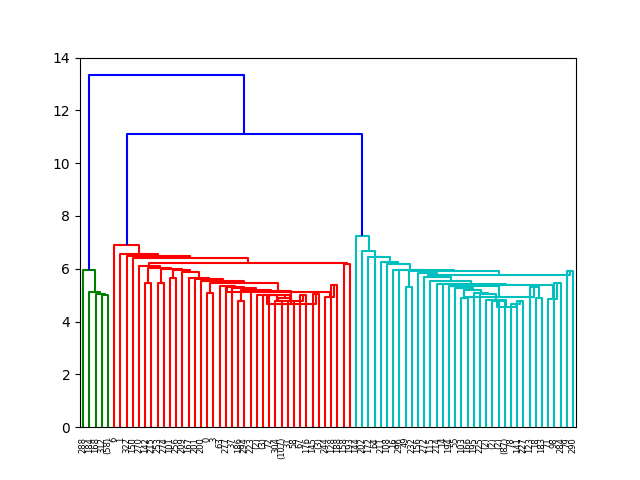
\includegraphics[width=16cm]{assets/hw_06_dendrogram.png}
\end{center}
While I was able to implement dendrogram data generation in my agglomeration
algorithm, I was not able to get it properly display in \texttt{scipy}. I used
\texttt{scipy}'s \texttt{linkage()} method to generate this dendrogram. See
the comments in the agglomeration algorithm for further details.

\begin{center}
  If you have any questions, comments, or concerns, please contact me at
  alvin@omgimanerd.tech
\end{center}

\end{document}
